\documentclass[10pt]{beamer}\usepackage[]{graphicx}\usepackage[]{color}
%% maxwidth is the original width if it is less than linewidth
%% otherwise use linewidth (to make sure the graphics do not exceed the margin)
\makeatletter
\def\maxwidth{ %
  \ifdim\Gin@nat@width>\linewidth
    \linewidth
  \else
    \Gin@nat@width
  \fi
}
\makeatother

\definecolor{fgcolor}{rgb}{0.345, 0.345, 0.345}
\newcommand{\hlnum}[1]{\textcolor[rgb]{0.686,0.059,0.569}{#1}}%
\newcommand{\hlstr}[1]{\textcolor[rgb]{0.192,0.494,0.8}{#1}}%
\newcommand{\hlcom}[1]{\textcolor[rgb]{0.678,0.584,0.686}{\textit{#1}}}%
\newcommand{\hlopt}[1]{\textcolor[rgb]{0,0,0}{#1}}%
\newcommand{\hlstd}[1]{\textcolor[rgb]{0.345,0.345,0.345}{#1}}%
\newcommand{\hlkwa}[1]{\textcolor[rgb]{0.161,0.373,0.58}{\textbf{#1}}}%
\newcommand{\hlkwb}[1]{\textcolor[rgb]{0.69,0.353,0.396}{#1}}%
\newcommand{\hlkwc}[1]{\textcolor[rgb]{0.333,0.667,0.333}{#1}}%
\newcommand{\hlkwd}[1]{\textcolor[rgb]{0.737,0.353,0.396}{\textbf{#1}}}%
\let\hlipl\hlkwb

\usepackage{framed}
\makeatletter
\newenvironment{kframe}{%
 \def\at@end@of@kframe{}%
 \ifinner\ifhmode%
  \def\at@end@of@kframe{\end{minipage}}%
  \begin{minipage}{\columnwidth}%
 \fi\fi%
 \def\FrameCommand##1{\hskip\@totalleftmargin \hskip-\fboxsep
 \colorbox{shadecolor}{##1}\hskip-\fboxsep
     % There is no \\@totalrightmargin, so:
     \hskip-\linewidth \hskip-\@totalleftmargin \hskip\columnwidth}%
 \MakeFramed {\advance\hsize-\width
   \@totalleftmargin\z@ \linewidth\hsize
   \@setminipage}}%
 {\par\unskip\endMakeFramed%
 \at@end@of@kframe}
\makeatother

\definecolor{shadecolor}{rgb}{.97, .97, .97}
\definecolor{messagecolor}{rgb}{0, 0, 0}
\definecolor{warningcolor}{rgb}{1, 0, 1}
\definecolor{errorcolor}{rgb}{1, 0, 0}
\newenvironment{knitrout}{}{} % an empty environment to be redefined in TeX

\usepackage{alltt}

%% include header:
\usetheme{metropolis}
\usepackage{appendixnumberbeamer}

\usepackage{booktabs}
\usepackage[scale=2]{ccicons}

\usepackage{pgfplots}
\usepgfplotslibrary{dateplot}

\usepackage{xspace}
\newcommand{\themename}{\textbf{\textsc{metropolis}}\xspace}

\usepackage[english]{babel}
\usepackage{dsfont}
\usepackage{amsmath}
\usepackage{amssymb}
\usepackage{amsthm}
\usepackage{amsfonts}


%% Define theme color(s):
%% ---------------------------------------------------------------

\usepackage{xcolor}

\definecolor{metropolis_theme_color}{RGB}{35,55,59}
% \definecolor{metropolis_theme_color}{RGB}{110, 117, 87}

%% Color custimzations:
\definecolor{blue}{RGB}{0,155,164}
\definecolor{lime}{RGB}{175,202,11}
\definecolor{green}{RGB}{0,137,62}
\definecolor{titleblue}{RGB}{112,122,82}
\definecolor{deepskyblue}{RGB}{0,191,255}
\definecolor{mygrey}{RGB}{240,240,240}

% \setbeamercolor{progress bar}{fg=deepskyblue}
% \setbeamercolor{frametitle}{bg=metropolis_theme_color}

%% Shaded for nicer code highlighting:
%% ---------------------------------------------------------------

\usepackage{mdframed}
% \usepackage{verbatim}

% Define Shaded if not defined:
\makeatletter
\@ifundefined{Shaded}{%
  \newenvironment{Shaded}{\begin{snugshade}}{\end{snugshade}}%
}{}
\makeatother

\renewenvironment{Shaded}{
  \begin{mdframed}[
    backgroundcolor=mygrey,
    linecolor=metropolis_theme_color,
    rightline=false,
		leftline=false
  ]}{
  \end{mdframed}
}

%% Title Image:
%% ---------------------------------------------------------------

% Load transparent:
\usepackage{transparent}

% Add titlegraphic:
\titlegraphic{
  \vspace{2cm}
  \hspace{5.03cm}
  \transparent{0.2}
  
\includegraphics[width=8cm]{images/logos/LMU}
}

%% Adjust frame number to be displayd as i/n:
%% ---------------------------------------------------------------
\setbeamertemplate{frame numbering}{%
  \insertframenumber{}/\inserttotalframenumber
}
\makeatother


%% Include latex-math:
%% ---------------------------------------------------------------
% Include latex-math
\DeclareOldFontCommand{\sf}{\normalfont\sffamily}{\mathsf}

\IfFileExists{./latex-math/basic-math.tex}{
  \input{./latex-math/basic-math.tex}
  \input{./latex-math/ml-bagging.tex}
  \input{./latex-math/ml-boosting.tex}
  \input{./latex-math/ml-gp.tex}
  \input{./latex-math/ml-mbo.tex}
  \input{./latex-math/ml-nn.tex}
  \input{./latex-math/ml-svm.tex}
  \input{./latex-math/ml-trees.tex}
}{
  \IfFileExists{./../latex-math/basic-math.tex}{
    \input{./../latex-math/basic-math.tex}
    \input{./../latex-math/basic-ml.tex}
    \input{./../latex-math/ml-bagging.tex}
    \input{./../latex-math/ml-boosting.tex}
    \input{./../latex-math/ml-gp.tex}
    \input{./../latex-math/ml-mbo.tex}
    \input{./../latex-math/ml-nn.tex}
    \input{./../latex-math/ml-svm.tex}
    \input{./../latex-math/ml-trees.tex}
  }{}
}

%% Style URLs
%% ---------------------------------------------------------------

\usepackage{hyperref}

\definecolor{myorange}{RGB}{225, 127, 0}
\renewcommand\UrlFont{\color{myorange}}

%% include template:
%% Footer:
\usepackage{xfrac}
\usepackage{framed, color}

\setbeamertemplate{footline}[text line]{%
    \noindent\hspace*{\dimexpr-\oddsidemargin-1in\relax}%
     \colorbox{metropolis_theme_color}{
     \makebox[\dimexpr\paperwidth-2\fboxsep\relax]{
     \color{mygrey}
     \begin{minipage}{0.33\linewidth}
       \secname
     \end{minipage}\hfill
     \begin{minipage}{0.33\linewidth}
       \centering
       \insertshortauthor
     \end{minipage}\hfill
     \begin{minipage}{0.33\linewidth}
       \flushright
       \insertframenumber{}/\inserttotalframenumber
     \end{minipage}     
     }}%
  \hspace*{-\paperwidth}
}

%% Custom stuff:
\usepackage[]{algorithm2e}
\usepackage{csquotes}
\usepackage{dsfont}

%% Title:
%% ----------------------------------------

\title{Compboost}
\subtitle{Modular framework for component-wise boosting}
\date{\today}
\author{Daniel Schalk}
\institute{LMU Munich\\Working Group Computational Statistics}

%% Wrap Shaded around Shunk to have a nices R output:
%% --------------------------------------------------

% Include before begin document to have Schunk:

\let\Oldkframe\kframe
\let\endOldkframe\endkframe

\renewenvironment{kframe}
 {\scriptsize\definecolor{shadecolor}{RGB}{240,240,240}\begin{Shaded}\Oldkframe}
 {\endOldkframe\end{Shaded}\normalsize}

%% Prevent code from printing over margin:
%% --------------------------------------------------
 


%% Content:
%% ----------------------------------------
\IfFileExists{upquote.sty}{\usepackage{upquote}}{}
\begin{document}




\maketitle

\begin{frame}[plain]{Table of contents}
	\setbeamertemplate{section in toc}[sections numbered]
	\tableofcontents[hideallsubsections]
\end{frame}


\section{What is Component-Wise Boosting}


\begin{frame}[fragile]{Component-Wise Boosting: Terminology}


\begin{itemize}

  \item
    Loss Function: 
    \[
      L: \mathcal{Y} \times \mathcal{X} \rightarrow \mathbb{R}
    \]

  \item
    Empirical Risk:
    \[
      \riske(\theta) = \frac{1}{n} \sumin L\left(\yi, f(\xi)\right)
    \]

  \item 
    Estimated model/parameter at iteration $m$: 
    \[
      \fmh, \theta^{[m]}
    \]

\end{itemize}


\end{frame}



\begin{frame}[fragile]{Component-Wise Boosting: The Idea}

\begin{figure}
\centering
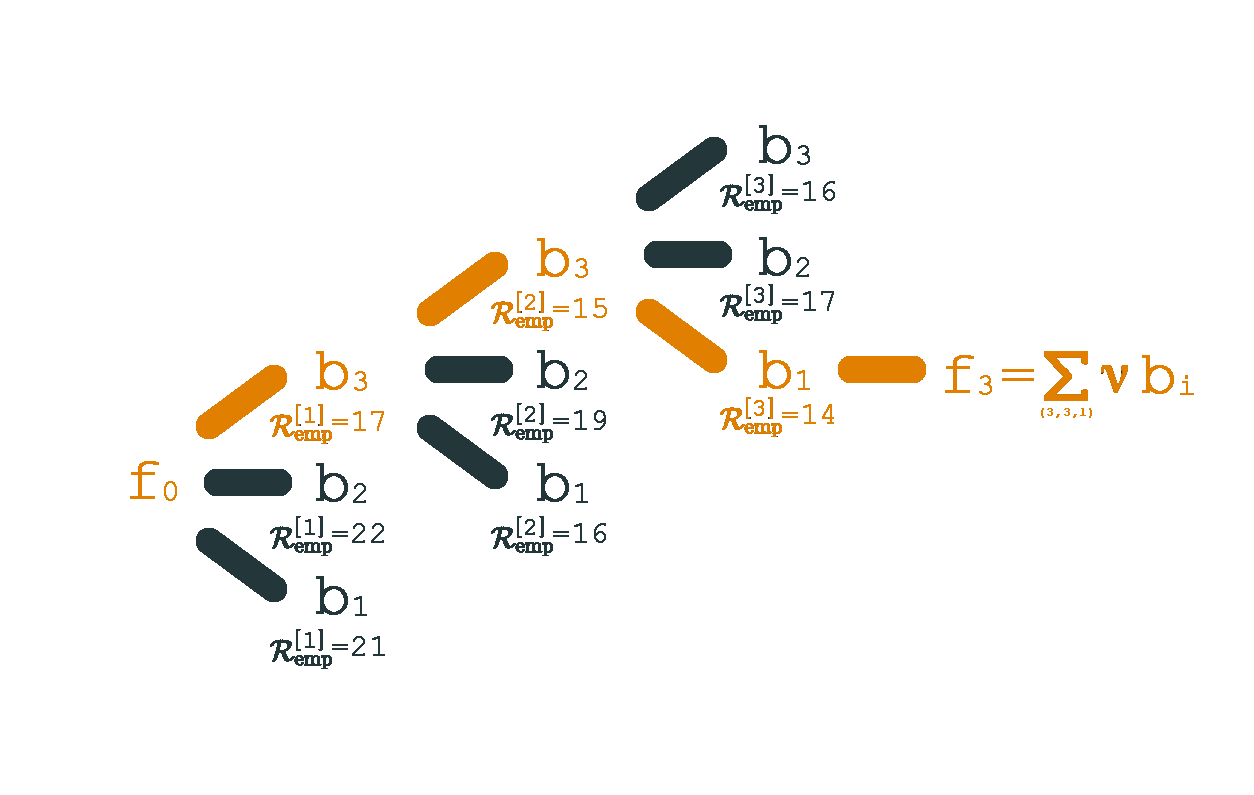
\includegraphics[width=0.7\textwidth]{images/comp_boosting.png}
\end{figure}

\vspace{-1.5cm}

\begin{align*}
  \text{Iteration 1:} \ &\hat{f}^{[1]}(x) = \beta b_3(x_3, \theta^{[1]}) \\
  \text{Iteration 2:} \ &\hat{f}^{[2]}(x) = \beta b_3(x_3, \theta^{[1]}) + \beta b_3(x_3, \theta^{[2]}) \\
  \text{Iteration 2:} \ &\hat{f}^{[3]}(x) = \beta b_3(x_3, \theta^{[1]}) + \beta b_3(x_3, \theta^{[2]}) + \beta b_1(x_1, \theta^{[3]}) \\ \\
  \Rightarrow\ &\hat{f}^{[3]}(x) = \beta \left( b_3(x_3, \theta^{[1]} + \theta^{[2]}) + b_1(x_1, \theta^{[3]}) \right)
\end{align*}


\end{frame}



\begin{frame}{Component-Wise Boosting: The Algorithm}

\begin{Shaded}
\begin{algorithm}[H]
% \KwData{this text}
\scriptsize
\KwResult{Component-wise boosting model $\fh(x)$}
Initialize $\fh^{[0]}(x) = \argmin_{c\in\R} \riske(c)$ \;
  \For{$m \in \{1, \dots, M\}$}{\vspace{0.2cm}
    // Update pseudo residuals: \\
    $r^{[m](i)} = -\left[ \frac{\delta}{\delta f(\xi)} L\left(\yi, f(\xi)\right) \right]_{f = f^{[m-1]}},\ \forall i \in \{1, \dots, n\}$ \;\vspace{0.2cm}
    // Get index $j^\ast$ of $m$-th base-learner from optimizer:\\
    \For{$j \in \{1, \dots, J\}$}{
      // Fit each base-learner $b_j^{[m]}$ to the pseudo residuals: \\
      $\hat{\theta}_j^{[m]} = \argmin_{\theta_j} \sum\limits_{i=1}^n\left( 
      \rmi - b_j^{[m]}(\xi, \theta_j)\right)^2$ \;\vspace{0.2cm}
      // Calculate the SSE of the fitted base-learner:\\
      $\mathsf{SSE}_j = \sum\limits_{i=1}^n \left(\rmi - b_j^{[m]}(\xi, \hat{\theta}_j)\right)^2$ \; 
    }
    // Add selected component to model:\\
    $\fmh(x) = \fmdh(x) + \beta b^{[m]}_{j^\ast}\left(x, \theta_{j^\ast}^{[m]}\right)$
  }
\textbf{Returns:} $\fh(x) = \fmh(x)$\;
\end{algorithm}
\end{Shaded}

\end{frame}


\begin{frame}[fragile]{Available R Packages}

\begin{itemize}
	\item Tree-based implementations:
  \begin{itemize}
    \item \texttt{xgboost}
    \item \texttt{catboost}
    \item \texttt{gbm}
  \end{itemize}
  \item Model-based implementations:
  \begin{itemize}
    \item \texttt{mboost}
	\end{itemize}

\end{itemize}

So, why another boosting implementation?

\end{frame}


% \begin{frame}{}

% \begin{frame}[fragile]{R Plot Chunks}

% To include a \alert{centered plot}, \texttt{Sweave} you need to wrap
% \texttt{center} environment:

% \begin{center}
% <<echo=FALSE,fig=TRUE,height=4>>=
% library(ggplot2)
% ggplot(faithfuld, aes(waiting, eruptions, z = density)) +
%   geom_raster(aes(fill = density)) +
%   geom_contour(colour = "white")
% @
% \end{center}

% \end{frame}

% \begin{frame}{URLs}

% URLs can be easily included by \texttt{\textbackslash url\{myurl\}} and are illustrated in
% orange:
% \begin{center}
%   \url{https://mlr-org.github.io/mlr-tutorial/devel/html/}
% \end{center}
% \end{frame}


\section{About Compboost}


\begin{frame}[fragile]{About Compboost}

\begin{itemize}

	\item Installation
\begin{knitrout}
\definecolor{shadecolor}{rgb}{0.969, 0.969, 0.969}\color{fgcolor}\begin{kframe}
\begin{alltt}
\hlstd{devtools}\hlopt{::}\hlkwd{install_github}\hlstd{(}\hlstr{"schalkdaniel/compboost"}\hlstd{)}
\hlkwd{library}\hlstd{(compboost)}
\end{alltt}
\end{kframe}
\end{knitrout}


\end{itemize}

\end{frame}


\begin{frame}[fragile]{Compboost Members and Member Functions}

\begin{itemize}

	\item \textbf{Member Functions}:
	\begin{itemize}
	
	  \item \texttt{addBaselearner()}
	  \item \texttt{addLogger()}
	  \item \texttt{train()}
	  \item \texttt{coef()}
	  \item \texttt{predict()}
	  \item \texttt{risk()}
	  \item \texttt{selected()}
	  \item \texttt{plot()}
	  \item \texttt{...}

	\end{itemize}
  
	\item \textbf{Public Members}:
  \begin{itemize}
	
	  \item \texttt{model}
	  \item \texttt{bl.factory.list}
	  \item \texttt{loss}
	  \item \texttt{optimizer}
	  \item \texttt{...}

	\end{itemize}

\end{itemize}

\end{frame}

\section{Small Usecase}


\begin{frame}[fragile]{Initializng Model}

\begin{knitrout}
\definecolor{shadecolor}{rgb}{0.969, 0.969, 0.969}\color{fgcolor}\begin{kframe}
\begin{alltt}
\hlstd{mtcars}\hlopt{$}\hlstd{mpg_cat} \hlkwb{=} \hlkwd{ifelse}\hlstd{(mtcars}\hlopt{$}\hlstd{mpg} \hlopt{>} \hlnum{15}\hlstd{,} \hlstr{"A"}\hlstd{,} \hlstr{"B"}\hlstd{)}
\hlstd{cboost} \hlkwb{=} \hlstd{Compboost}\hlopt{$}\hlkwd{new}\hlstd{(mtcars,} \hlstr{"mpg"}\hlstd{,} \hlkwc{loss} \hlstd{= QuadraticLoss}\hlopt{$}\hlkwd{new}\hlstd{())}

\hlstd{cboost}\hlopt{$}\hlkwd{addBaselearner}\hlstd{(}\hlstr{"wt"}\hlstd{,} \hlstr{"spline"}\hlstd{, PSplineBlearnerFactory,}
        \hlkwc{degree} \hlstd{=} \hlnum{3}\hlstd{,} \hlkwc{knots} \hlstd{=} \hlnum{10}\hlstd{,} \hlkwc{penalty} \hlstd{=} \hlnum{2}\hlstd{,} \hlkwc{differences} \hlstd{=} \hlnum{2}\hlstd{)}
\hlstd{cboost}\hlopt{$}\hlkwd{addBaselearner}\hlstd{(}\hlstr{"mpg_cat"}\hlstd{,} \hlstr{"linear"}\hlstd{, PolynomialBlearnerFactory,}
        \hlkwc{degree} \hlstd{=} \hlnum{1}\hlstd{,} \hlkwc{intercept} \hlstd{=} \hlnum{FALSE}\hlstd{)}

\hlstd{cboost}\hlopt{$}\hlkwd{train}\hlstd{(}\hlnum{2000}\hlstd{,} \hlkwc{trace}\hlstd{=}\hlnum{FALSE}\hlstd{)}
\hlstd{cboost}
\end{alltt}
\begin{verbatim}
## Componentwise Gradient Boosting
## 
## Trained on mtcars with target mpg
## Number of base-learners: 3
## Learning rate: 0.05
## Iterations: 2000
## Offset:20.090625
## 
## QuadraticLoss Loss:
## 
##   Loss function: y = (y - f(x))^2
## 
## 
\end{verbatim}
\end{kframe}
\end{knitrout}


\end{frame}

\begin{frame}[fragile]{Plot Results}

\begin{knitrout}
\definecolor{shadecolor}{rgb}{0.969, 0.969, 0.969}\color{fgcolor}\begin{kframe}
\begin{alltt}
\hlkwd{library}\hlstd{(ggplot2)}
\hlkwd{library}\hlstd{(ggthemes)}

\hlstd{cboost}\hlopt{$}\hlkwd{plot}\hlstd{(}\hlstr{"wt_spline"}\hlstd{,} \hlkwc{iters} \hlstd{=} \hlkwd{c}\hlstd{(}\hlnum{100}\hlstd{,} \hlnum{500}\hlstd{,} \hlnum{1000}\hlstd{,} \hlnum{2000}\hlstd{))} \hlopt{+}
        \hlkwd{labs}\hlstd{(}\hlkwc{title} \hlstd{=} \hlstr{"Effect of Weight"}\hlstd{,}
                \hlkwc{subtitle} \hlstd{=} \hlstr{"Additive contribution of linear predictor"}\hlstd{)} \hlopt{+}
        \hlkwd{theme_tufte}\hlstd{()} \hlopt{+}
        \hlkwd{scale_color_brewer}\hlstd{(}\hlkwc{palette} \hlstd{=} \hlstr{"Spectral"}\hlstd{)}
\end{alltt}
\end{kframe}
\end{knitrout}

\end{frame}


\begin{frame}[fragile]{Plot Results}

\begin{center}
\begin{knitrout}
\definecolor{shadecolor}{rgb}{0.969, 0.969, 0.969}\color{fgcolor}
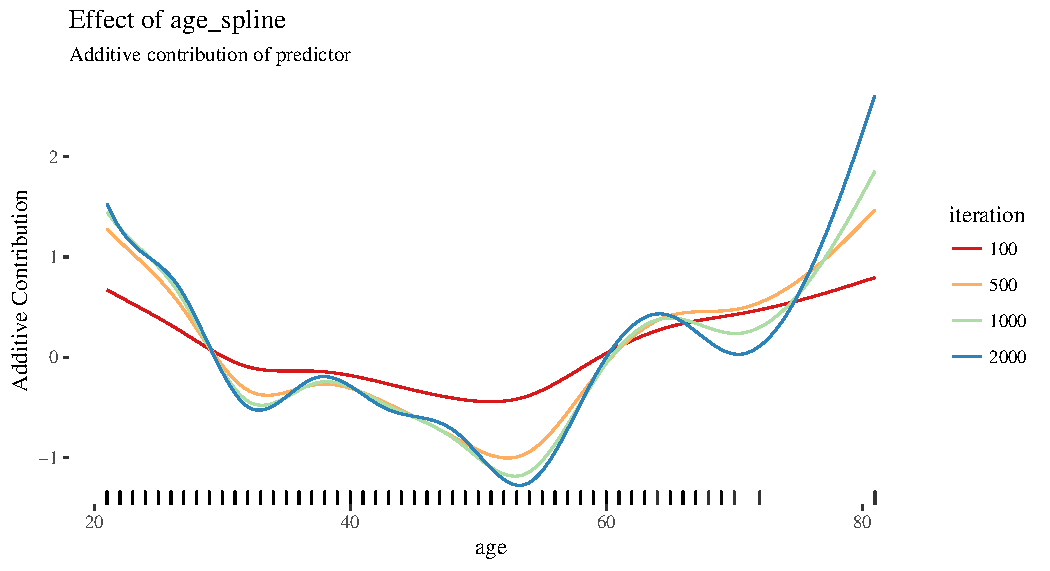
\includegraphics[width=11cm,height=6cm]{figure/unnamed-chunk-11-1} 

\end{knitrout}
\end{center}

\end{frame}
  
  
  \section{Next Steps}


\begin{frame}{}



\end{frame}



\begin{frame}[plain, standout]
  Questions?
\end{frame}


\end{document}
